\section{Le code de l'application}

\begin{minted}[frame=lines, linenos, fontsize=\small]{python}
import streamlit as st
import os
import json
import clip
import torch
from PIL import Image
import numpy as np

# Configuration
st.set_page_config(layout="wide")
images_folder = "images/4" # à modifier si besoin
json_folder = "clip_json"

# Charger le modèle CLIP
@st.cache_resource
def load_clip_model():
    device = "cuda" if torch.cuda.is_available() else "cpu"
    model, preprocess = clip.load("ViT-B/32", device=device)
    return model, preprocess, device

model, preprocess, device = load_clip_model()

# Charger les embeddings
@st.cache_data
def load_embeddings():
    embeddings = []
    for json_file in os.listdir(json_folder):
        if json_file.endswith(".json"):
            with open(os.path.join(json_folder, json_file), "r", encoding="utf-8") as f:
                data = json.load(f)
                embeddings.append({
                    "filename": data["filename"],
                    "embedding": np.array(data["embedding"]).astype("float32")
                })
    return embeddings

data = load_embeddings()

# Interface
st.title("Recherche visuelle d'images du RETIF avec CLIP")
# Texte d'introduction
st.text(
    "Bienvenue sur l'application Streamlit pour rechercher des images du RETIF grâce à CLIP !\n"
    "Assurez-vous d'avoir téléchargé les images et préparé les embeddings avec CLIP."
)

col1, col2 = st.columns(2)

# Recherche textuelle
with col1:
    text_query = st.text_input("Recherche par mots-clés (ex : pyramid, dog...)")

# Recherche par image
with col2:
    uploaded_image = st.file_uploader("Ou uploadez une image pour chercher par contenu", type=["jpg", "jpeg", "png"])

# Résultats
if not text_query and not uploaded_image:
    st.info("Entrez un mot-clé ou uploadez une image pour lancer une recherche.")
else:
    if text_query:
        with torch.no_grad():
            tokens = clip.tokenize([text_query]).to(device)
            text_features = model.encode_text(tokens)
            text_features /= text_features.norm(dim=-1, keepdim=True)
            query_vector = text_features.cpu().numpy()[0]
        st.subheader(f"Résultats pour : *{text_query}*")

    elif uploaded_image:
        try:
            pil_img = Image.open(uploaded_image).convert("RGB")
            # Affichage dans la colonne 2
            with col2:
                st.image(pil_img, caption="Image envoyée", width='stretch')
            image_input = preprocess(pil_img).unsqueeze(0).to(device)
            with torch.no_grad():
                image_features = model.encode_image(image_input)
                image_features /= image_features.norm(dim=-1, keepdim=True)
                query_vector = image_features.cpu().numpy()[0]
            st.subheader("Résultats similaires à l’image")
        except Exception as e:
            st.error(f"Erreur avec l’image envoyée : {e}")
            st.stop()

    # Recherche par similarité
    results = []
    for item in data:
        score = np.dot(query_vector, item["embedding"])
        results.append((score, item["filename"]))

    # Trier et afficher
    results.sort(reverse=True)
    cols = st.columns(5)
    for idx, (score, filename) in enumerate(results[:50]):
        with cols[idx % 5]:

            st.image(os.path.join(images_folder, filename), caption=f"{filename}\nScore: {score:.2f}", width='stretch')
            
\end{minted}


\section{Visuels de l'application Streamlit}

\begin{figure}[H]
    \centering
    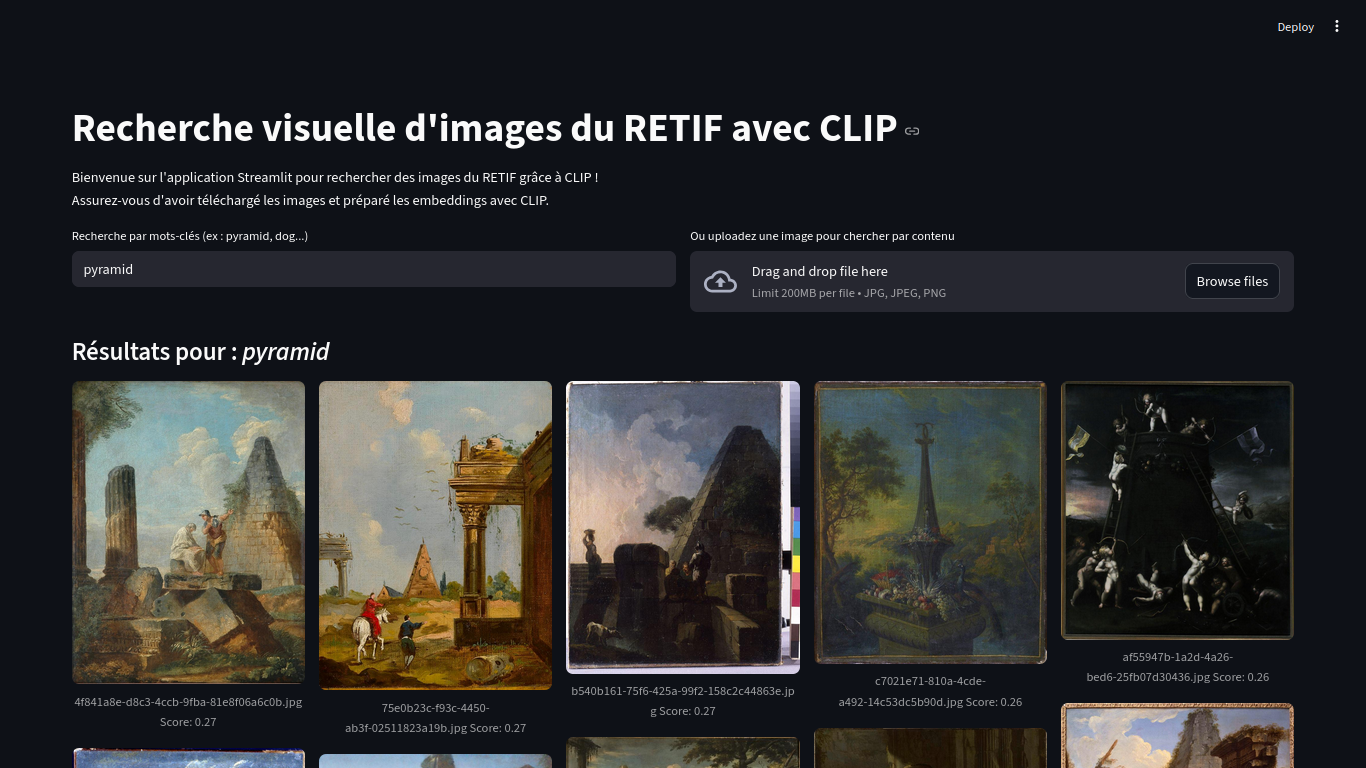
\includegraphics[width=1\textwidth]{annexes/figures/APP-pyramid.png}
    \caption{Recherche du terme "pyramid" dans le moteur de recherche CLIP de l'application}
    \label{fig:APP-pyramid}
\end{figure}

\begin{figure}[H]
    \centering
    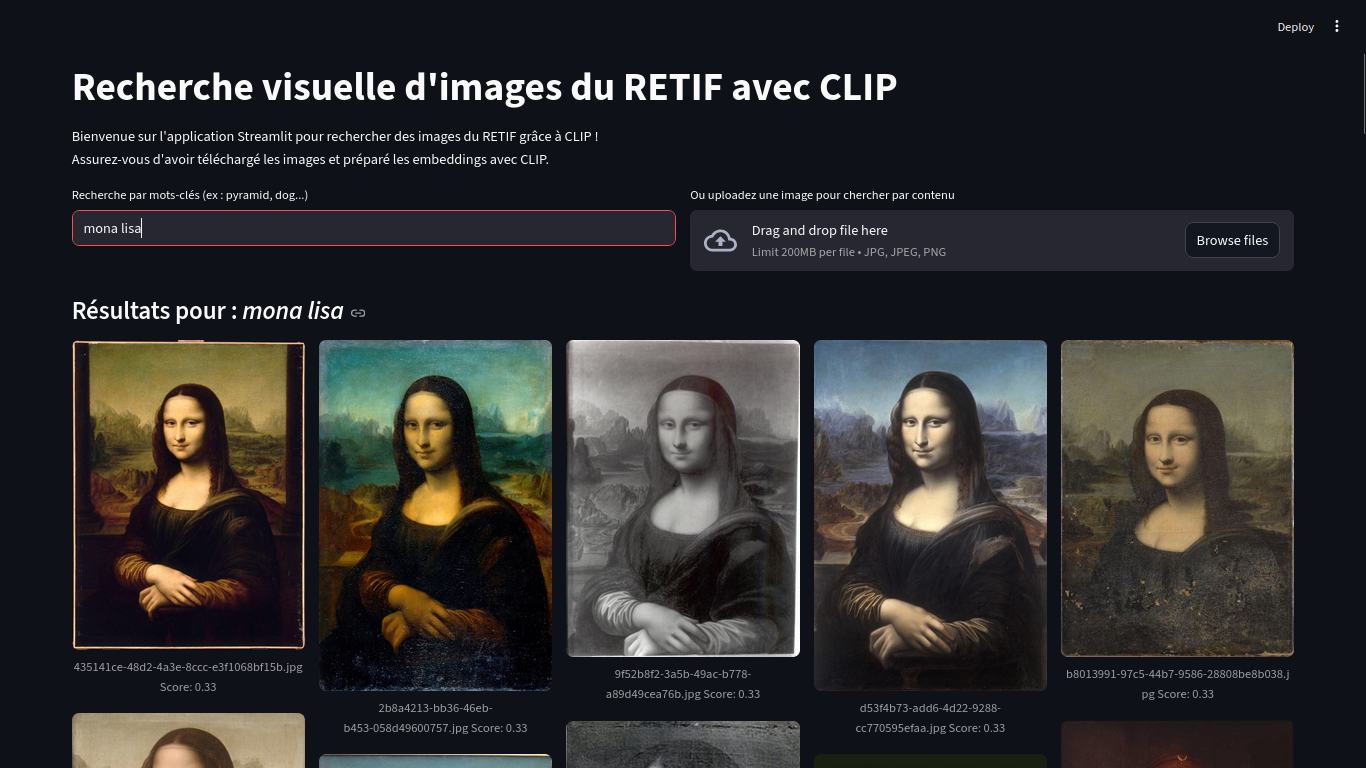
\includegraphics[width=1\textwidth]{annexes/figures/APP-monalisa.png}
    \caption{Recherche des termes "mona lisa" dans le moteur de recherche CLIP de l'application}
    \label{fig:APP-monalisa}
\end{figure}

\begin{figure}[H]
    \centering
    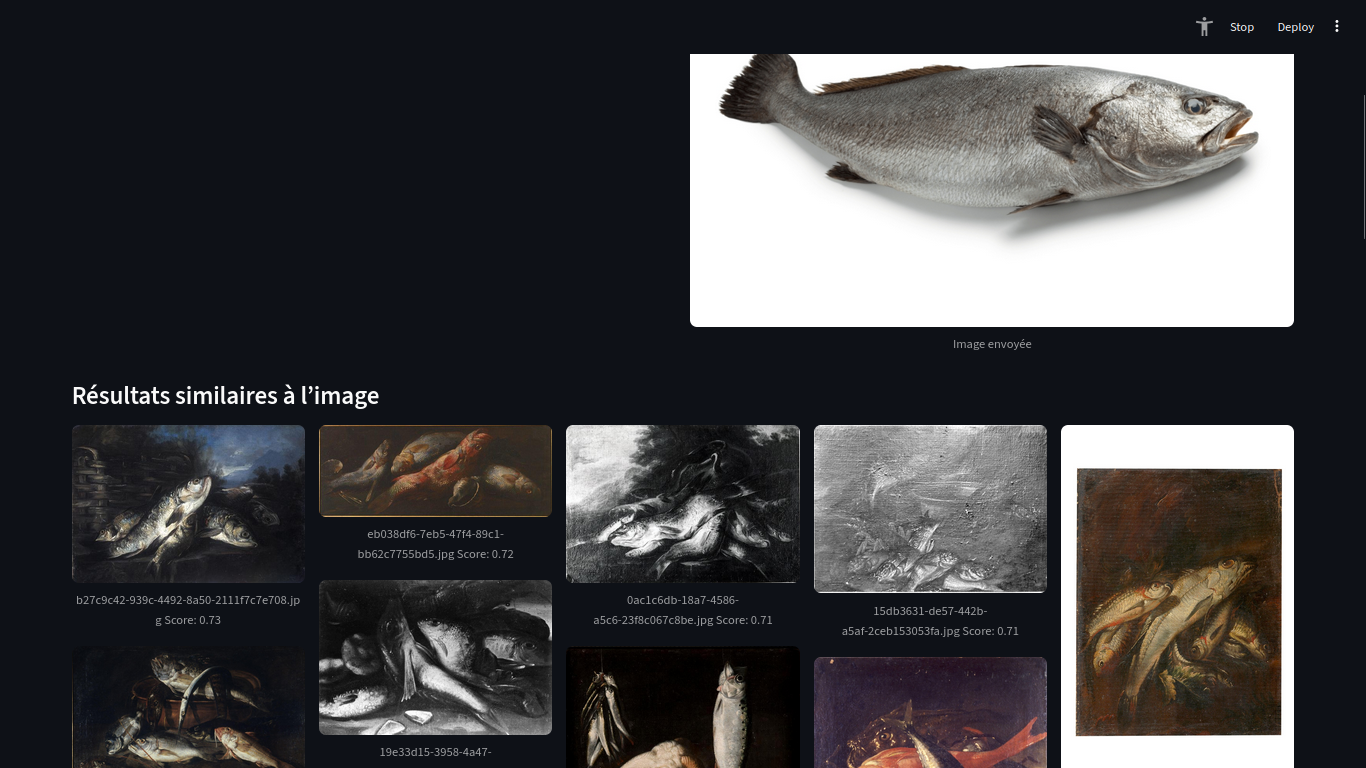
\includegraphics[width=1\textwidth]{annexes/figures/APP-poisson.png}
    \caption{Recherche par image à l'aide d'une photographie d'un poisson dans le moteur de recherche CLIP de l'application}
    \label{fig:APP-poisson}
\end{figure}

\begin{figure}[H]
    \centering
    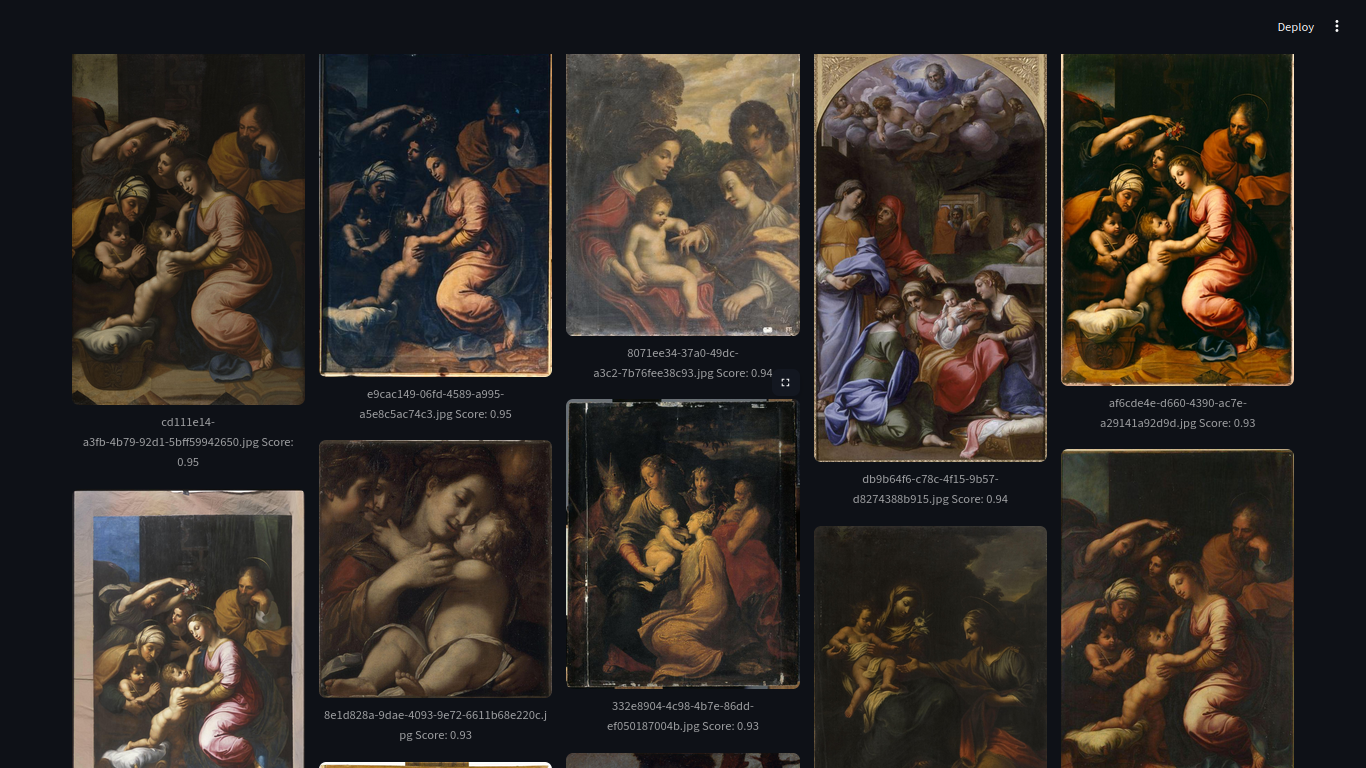
\includegraphics[width=1\textwidth]{annexes/figures/APP-raphael.png}
    \caption{Recherche par image à l'aide de la Sainte Famille de François 1er dans l'application (figure \ref{fig:ptrRaphaelSteFam}).}
    \label{fig:APP-raphael}
\end{figure}

